\documentclass[12pt]{article}

\usepackage{sbc-template}
\usepackage{graphicx,url}
\usepackage[utf8]{inputenc}
\usepackage[brazil]{babel}
\usepackage{amsmath}
\usepackage{algorithm}
\usepackage{algpseudocode}
\usepackage{float}
\usepackage{caption}
%\usepackage[latin1]{inputenc}

\sloppy

\title{Análise da Distribuição de Probabilidade do Custo de Desenvolvimento pelo Governo\\ Cálculo de Contagem de Função e Seus Riscos}

\author{Raphael M. S. Jesus\inst{1}}

\address{Programa de Pós-Graduação em Informática\\ Universidade Federal do Rio de Janeiro (UFRJ)\\
  Av. Athos da Silveira Ramos, 274 Prédio do CCMN - Cidade Universitária
Ilha do Fundão \\ Rio de Janeiro, Brasil CEP:21941-916
\nextinstitute
   Instituto Tércio Pacitti de Aplicações e Pesquisas Computacionais\\
  Universidade Federal do Rio de Janeiro (UFRJ)
  \email{raphael.mauricio@gmail.com}
}

\begin{document}

\maketitle

\begin{abstract}
  This article aims to analyze the use of function points in government projects and establish a standard calculation for the value of projects. The main focus is to establish a standard for the calculation closest to what would be ideal for a project with the determined points. The analysis includes Monte Carlo simulations and the use of probabilistic distributions to estimate costs and risks.
\end{abstract}

\begin{resumo}
  Este artigo visa analisar o uso de pontos de função em projetos do governo e estabelecer um cálculo padrão para o valor dos projetos. O foco principal é estabelecer um padrão para o cálculo mais próximo do que seria o ideal para um projeto com os pontos determinados. A análise inclui simulações de Monte Carlo e o uso de distribuições probabilísticas para estimar custos e riscos.
\end{resumo}

\section{Introdução}

O uso de pontos de função como uma métrica para estimar o tamanho e o esforço de desenvolvimento de software tem sido amplamente adotado tanto na indústria quanto no setor público. No contexto governamental, é crucial que as estimativas de custo sejam precisas e reflitam os riscos associados a variações nos preços e na complexidade técnica dos projetos. Este trabalho visa estabelecer um padrão para a estimativa de custos de desenvolvimento de software em projetos governamentais, utilizando simulações de Monte Carlo para analisar a distribuição de probabilidade dos custos. As fórmulas e métodos utilizados são baseados no \textit{Roteiro de Métricas de Software do SISP} v2.3 \cite{sisp}, conforme descrito no \textit{Guia de Contagem de Pontos de Função do SISP para Projetos Data Warehouse} \cite{guia-dw}, onde a utilização de pontos de função é essencial para padronizar a estimativa de custos e esforços em projetos de data warehouse no setor governamental.

\section{Metodologia}
A metodologia empregada neste estudo envolve a coleta de dados, a aplicação de fórmulas para o cálculo de pontos de função e a simulação de Monte Carlo para análise de riscos.

\subsection{Fórmulas Utilizadas}
As fórmulas utilizadas para o cálculo de pontos de função são baseadas na análise de complexidade e nas categorias de funções, conforme descrito a seguir:

\subsubsection{Cálculo do Valor Contratado}
O cálculo do valor contratado para cada item de serviço é dado por:

\begin{equation}
\text{Valor Contratado} = \text{Quantidade Contratada} \times \text{Valor Unitário}
\end{equation}

\subsubsection{Cálculo de Pontos de Função}

Os Pontos de Função (PF) são uma métrica de tamanho funcional para sistemas de software. O cálculo é realizado através das seguintes etapas, conforme descrito no \textit{Roteiro de Métricas de Software do SISP} v2.3 \cite{sisp}:

1. Identificação e classificação dos componentes do sistema (Entradas Externas, Saídas Externas, Consultas Externas, Arquivos Lógicos Internos e Arquivos de Interface Externa).

2. Atribuição de pesos a cada componente com base na sua complexidade.

3. Aplicação de um fator de ajuste que leva em consideração características gerais do sistema.

As fórmulas para o cálculo dos Pontos de Função são:

\begin{equation}
PF = (ILF \times \text{peso}_\text{ILF}) + (EIF \times \text{peso}_\text{EIF}) + (EI \times \text{peso}_\text{EI}) + (EO \times \text{peso}_\text{EO}) + (EQ \times \text{peso}_\text{EQ})
\end{equation}

\begin{equation}
PF_{\text{ajustado}} = PF \times (0.65 + 0.01 \times \sum_{i=1}^{14} F_i)
\end{equation}

Onde:
\begin{itemize}
    \item \textbf{ILF}: Arquivos Lógicos Internos
    \item \textbf{EIF}: Arquivos de Interface Externa
    \item \textbf{EI}: Entradas Externas
    \item \textbf{EO}: Saídas Externas
    \item \textbf{EQ}: Consultas Externas
    \item \textbf{F$_i$}: Características gerais do sistema (0 a 5)
    \item \textbf{peso$_x$}: Peso de cada componente com base na complexidade
\end{itemize}

\section{Algoritmo de Cálculo de Pontos de Função}

O algoritmo a seguir calcula os Pontos de Função ajustados conforme as fórmulas definidas pelo \textit{Roteiro de Métricas de Software do SISP} v2.3.

\begin{algorithm}[H]
\caption{Calcular Pontos de Função Ajustados}
\begin{algorithmic}[1]
\Procedure{calcularPontosFuncao}{$ILF, EIF, EI, EO, EQ, pesos, ajusteComplexidade$}
    \State $PF \gets (ILF \times pesos[ILF]) + (EIF \times pesos[EIF]) +$
    \State \hspace{3.5em} $(EI \times pesos[EI]) + (EO \times pesos[EO]) + (EQ \times pesos[EQ])$
    \State $PF\_ajustado \gets PF \times (0.65 + 0.01 \times ajusteComplexidade)$
    \State Escrever("Pontos de Função ajustados: ", $PF\_ajustado$)
\EndProcedure
\end{algorithmic}
\end{algorithm}

\subsection{Simulação de Monte Carlo}

A simulação de Monte Carlo é uma técnica utilizada para entender o impacto do risco e da incerteza em modelos e previsões. No contexto deste trabalho, utilizo a simulação de Monte Carlo para estimar os custos de desenvolvimento de software a partir de pontos de função, considerando variáveis como a experiência da equipe e a complexidade técnica.

\begin{algorithm}[H]
\caption{Calcular custo usando Monte Carlo}
\begin{algorithmic}[1]
\Procedure{calcular\_custo\_mc}{num\_pontos\_funcao, min\_preco, mode\_preco, max\_preco, experiencia\_equipe, complexidade\_tecnica, n\_simulacoes}
    \State custos $\leftarrow$ vetor de tamanho $n\_simulacoes$
    \For{$i = 1$ to $n\_simulacoes$}
        \State preco $\leftarrow$ rtriangle(1, a = min\_preco, b = max\_preco, c = mode\_preco)
        \State custo $\leftarrow$ preco $\times$ num\_pontos\_funcao $\times$ experiencia\_equipe $\times$ complexidade\_tecnica
        \State custos[i] $\leftarrow$ custo
    \EndFor
    \State \Return custos
\EndProcedure
\end{algorithmic}
\end{algorithm}

\subsection{Parâmetros Utilizados}

Para as simulações, foram utilizados os seguintes parâmetros baseados na análise de contratos governamentais \textit{via Portal da Transparencia}\cite{portal}:

\begin{itemize}
    \item \textbf{Número de Pontos de Função:} 500
    \item \textbf{Experiência da Equipe:} 1.1 (equivalente a uma equipe com experiência moderada)
    \item \textbf{Complexidade Técnica:} 1.2 (alta complexidade técnica)
    \item \textbf{Número de Simulações:} 10.000
\end{itemize}

Os valores para os preços mínimo, máximo e modal foram derivados de contratos reais, conforme a tabela a seguir:

\begin{table}[H]
\centering
\caption{Estimativas de Custos por Tipo de Desenvolvimento}
\resizebox{\textwidth}{!}{%
\begin{tabular}{|c|c|c|c|}
\hline
\textbf{Tipo de Desenvolvimento} & \textbf{Preço Mínimo} & \textbf{Preço Modal} & \textbf{Preço Máximo} \\
\hline
Novo Desenvolvimento & R\$ 5,000 & R\$ 10,000 & R\$ 20,000 \\
Manutenção & R\$ 3,000 & R\$ 7,000 & R\$ 15,000 \\
Adaptação & R\$ 2,000 & R\$ 5,000 & R\$ 10,000 \\
\hline
\end{tabular}%
}
\label{tab:precos}
\end{table}

\section{Resultados}

Os resultados da simulação de Monte Carlo mostraram a distribuição dos custos médios por ponto de função, como apresentado na Figura \ref{fig:distribuicao_custos}. Esta análise permitiu entender a variabilidade dos custos e os possíveis cenários de risco associados aos projetos de software no contexto governamental.

\begin{figure}[H]
\centering
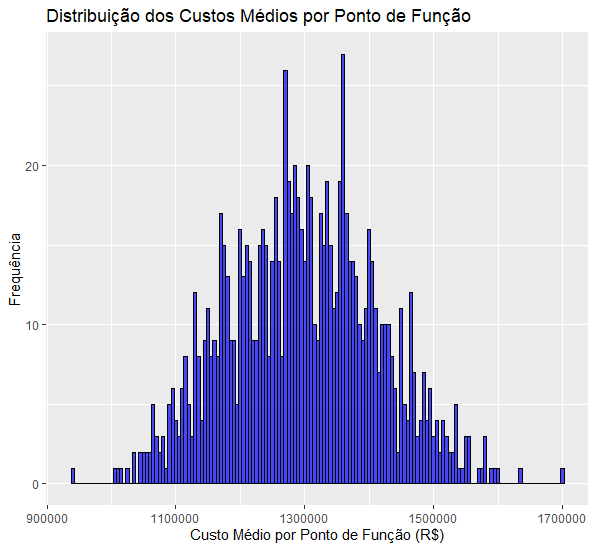
\includegraphics[width=0.7\textwidth]{custo_medio_pf.jpg}
\caption{Distribuição dos Custos Médios por Ponto de Função com Base nas Simulações de Monte Carlo}
\label{fig:distribuicao_custos}
\end{figure}

A Tabela \ref{tab:resultados_sensibilidade} resume a análise de sensibilidade dos custos médios por ponto de função, destacando os percentis 5\% e 95\%.

\begin{table}[H]
\centering
\caption{Análise de Sensibilidade dos Custos Médios por Ponto de Função}
\begin{tabular}{|c|c|}
\hline
\textbf{Percentil} & \textbf{Custo Médio por Ponto de Função (R\$)} \\
\hline
5\% & \text{1.110.234} \\
95\% & \text{1.491.692} \\
\hline
\end{tabular}
\label{tab:resultados_sensibilidade}
\end{table}

\section{Conclusão}
A aplicação de métodos de contagem de pontos de função e a simulação de Monte Carlo permite uma análise detalhada dos custos de desenvolvimento de software em projetos governamentais. O uso dessas técnicas ajuda a prever riscos e a tomar decisões informadas sobre alocação de recursos e planejamento de projetos. Futuras pesquisas podem explorar a aplicação desses métodos em diferentes contextos e com variáveis adicionais para melhorar ainda mais a precisão das estimativas.

\bibliographystyle{sbc}
\bibliography{sbc-template}

\end{document}